\section{Agent Architectures and Frameworks}
\label{sec:agent-architectures}

Building intelligent agents requires combining Large Language Models with structured reasoning patterns and tool integration frameworks. This section examines the ReAct agent architecture and the OpenAI Agents SDK, which form the foundation of the Slurm Agent implementation.

\subsection{ReAct: Reasoning and Acting}

The ReAct paradigm, introduced by Yao et al. \cite{yao2022react}, represents a significant advancement in LLM-based agent design. ReAct synergizes \textbf{reasoning} (generating verbal reasoning traces) with \textbf{acting} (taking actions that affect the environment), enabling agents to solve complex tasks that require both planning and external interaction.

\subsubsection{The Think-Act-Observe Loop}

ReAct agents operate through an iterative loop with three distinct phases:

\begin{enumerate}
    \item \textbf{Think}: The agent generates a reasoning trace explaining its current understanding and intended next step. This internal monologue helps decompose complex problems and maintain task focus.
    
    \item \textbf{Act}: Based on the reasoning, the agent selects and executes an action---typically invoking an external tool with specific parameters.
    
    \item \textbf{Observe}: The agent receives the result of its action from the environment and incorporates this observation into its context for the next iteration.
\end{enumerate}

This cycle repeats until the agent determines it has sufficient information to provide a final response, or encounters a termination condition.

\begin{figure}[H]
    \centering
    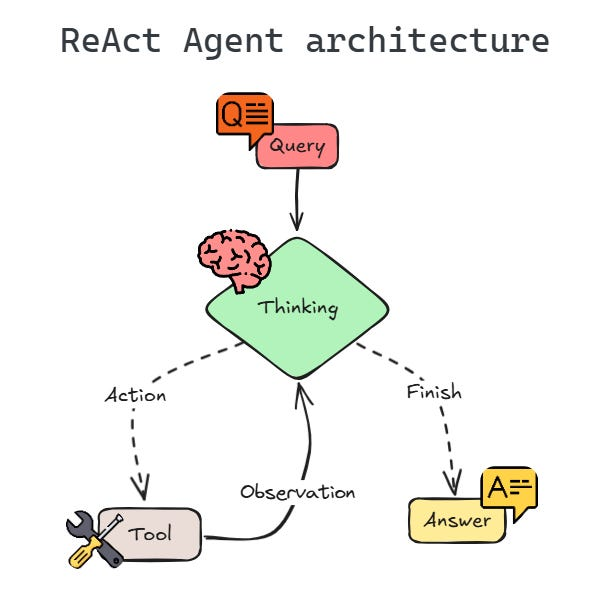
\includegraphics[width=0.5\textwidth]{images/react_agent_arch.png}
    \caption{The ReAct Think-Act-Observe Loop}
    \label{fig:react-loop}
\end{figure}

ReAct is suitable for HPC operations because: (1)~Slurm diagnosis requires chaining multiple queries (queue state, priority, partition availability) before concluding; (2)~the reasoning trace makes tool selections auditable; (3)~observations can revise the agent's plan when initial assumptions are wrong.

\subsection{OpenAI Agents SDK}

The OpenAI Agents SDK~\cite{openaiagentssdk2024} provides the execution framework used in this project. Its key abstractions are:

\begin{itemize}
    \item \textbf{Agent}: An LLM with instructions, tools, and behavioral config. Separate agents isolate read-only observation from state-changing operations.
    \item \textbf{Runner}: Manages the execution loop—sending messages, processing tool calls, collecting results.
    \item \textbf{Tools}: Functions agents invoke to interact with external systems, with automatic parameter validation.
    \item \textbf{Handoffs}: Transfer control between specialized agents, passing conversation context.
\end{itemize}

The Runner's internal loop naturally implements ReAct: (1)~collect messages, (2)~send to LLM, (3)~if tool calls, execute and loop; (4)~if final text, return; (5)~if handoff, transfer to target agent. The SDK also integrates with MCP servers, treating MCP tools as native agent tools.
